\subsection{DImage  Class Reference}
\label{class_dimage}\index{DImage@{DImage}}
a double precision image type. 


{\tt \#include $<$dimage.h$>$}

Inheritance diagram for DImage::\begin{figure}[H]
\begin{center}
\leavevmode
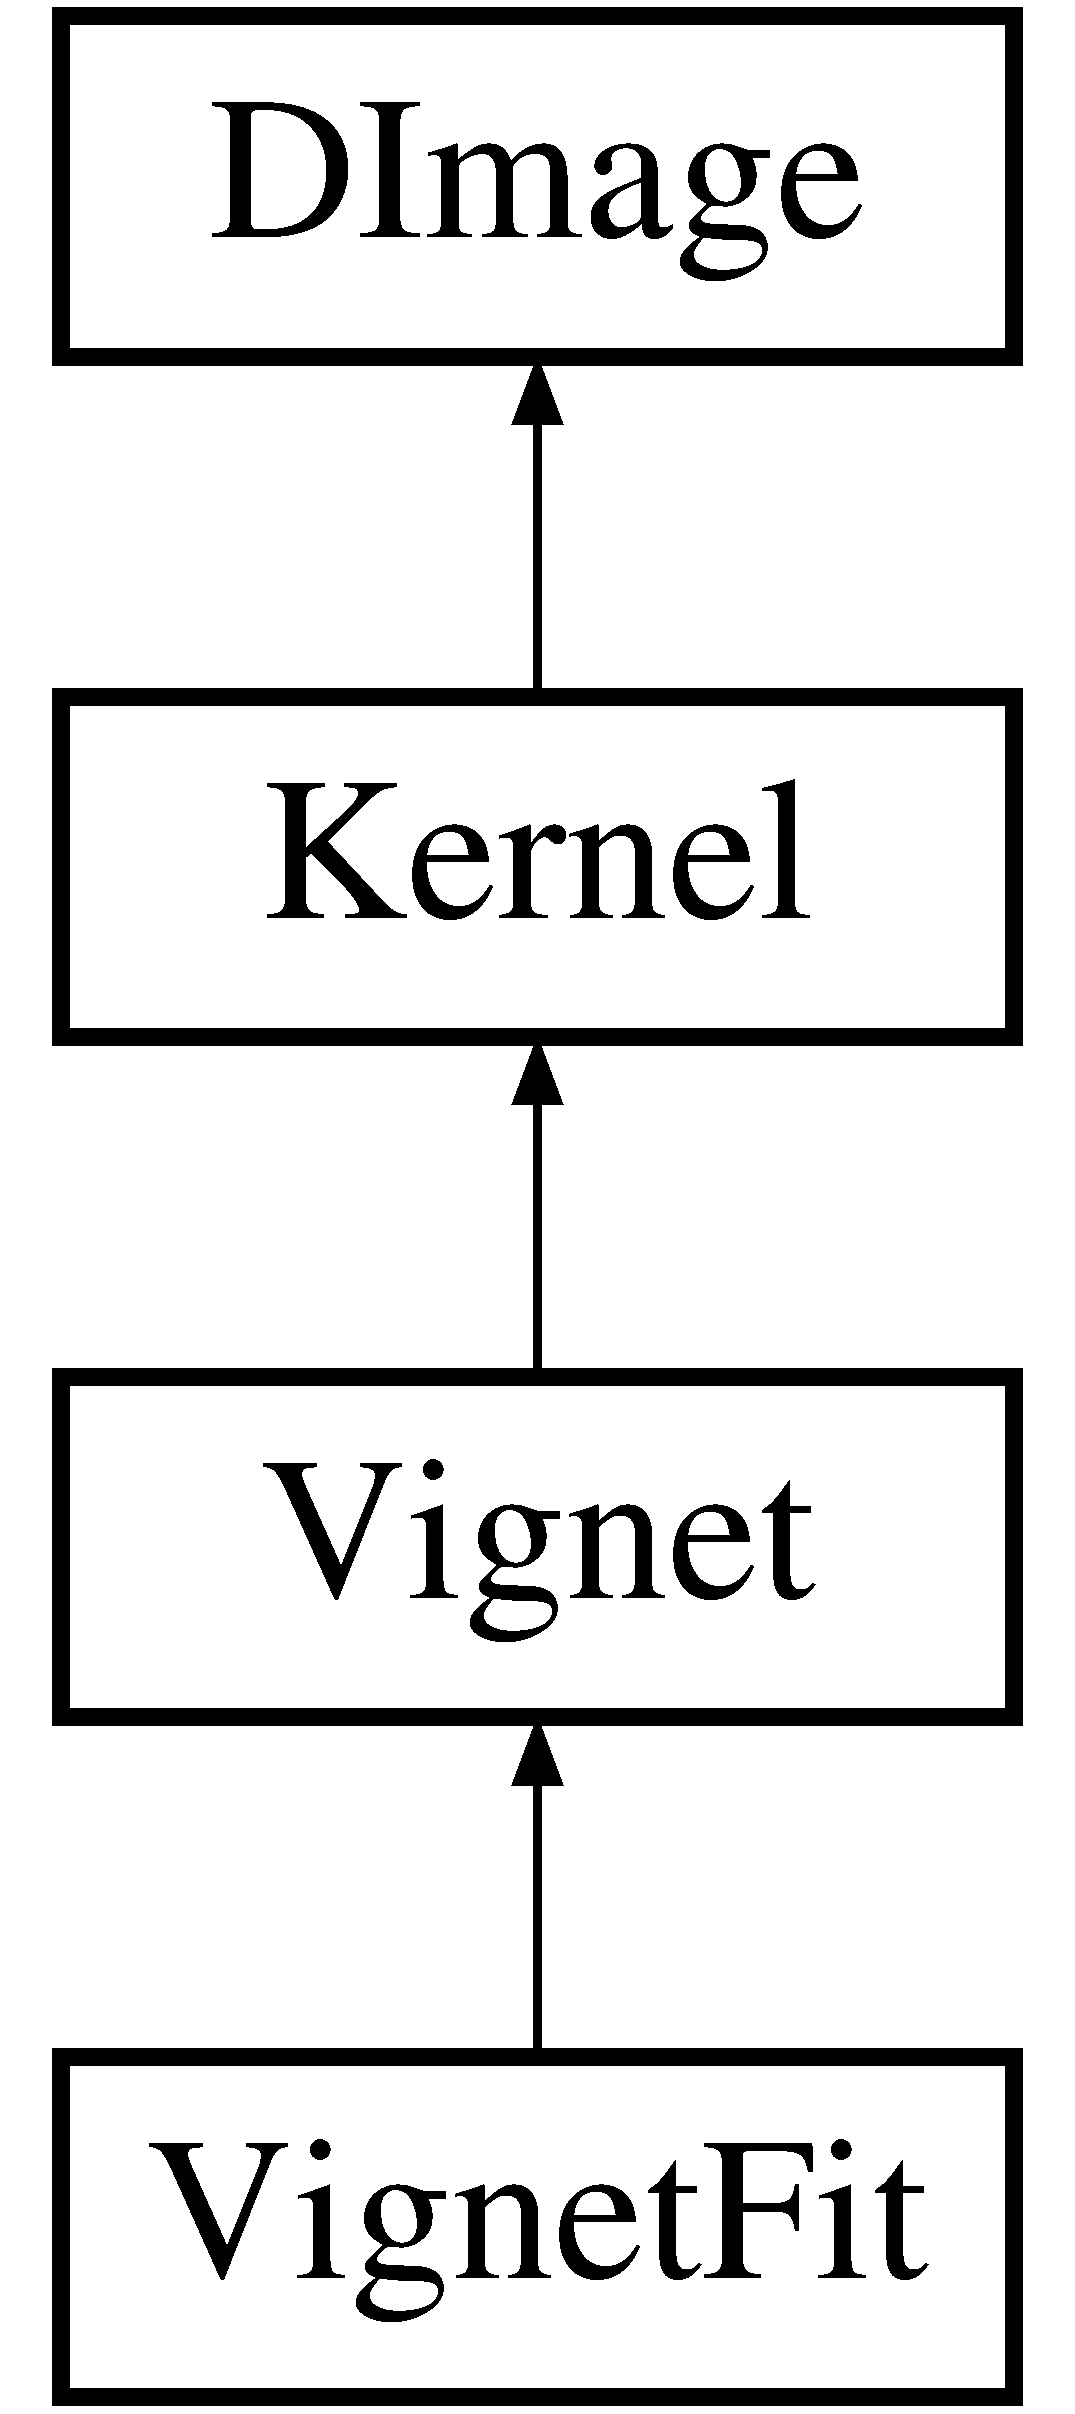
\includegraphics[height=4cm]{class_dimage}
\end{center}
\end{figure}
\subsubsection*{Public Methods}
\begin{CompactItemize}
\item 
\index{DImage@{DImage}!DImage@{DImage}}\index{DImage@{DImage}!DImage@{DImage}}
{\bf DImage} (const int Nx, const int Ny)\label{class_dimage_a0}

\item 
\index{DImage@{DImage}!DImage@{DImage}}\index{DImage@{DImage}!DImage@{DImage}}
{\bf DImage} ()\label{class_dimage_a1}

\item 
\index{Allocate@{Allocate}!DImage@{DImage}}\index{DImage@{DImage}!Allocate@{Allocate}}
void {\bf Allocate} (const int Nx, const int Ny, int Init=1)\label{class_dimage_a2}

\item 
\index{~DImage@{$\sim$DImage}!DImage@{DImage}}\index{DImage@{DImage}!~DImage@{$\sim$DImage}}
{\bf $\sim$DImage} ()\label{class_dimage_a3}

\item 
\index{operator()@{operator()}!DImage@{DImage}}\index{DImage@{DImage}!operator()@{operator()}}
DPixel\& {\bf operator()} (const int i, const int j) const\label{class_dimage_a4}

\begin{CompactList}\small\item\em value on (i,j).\item\end{CompactList}\item 
\index{begin@{begin}!DImage@{DImage}}\index{DImage@{DImage}!begin@{begin}}
DPixel$\ast$ {\bf begin} () const\label{class_dimage_a5}

\begin{CompactList}\small\item\em acces to pointer on first pixel of array.\item\end{CompactList}\item 
\index{Nx@{Nx}!DImage@{DImage}}\index{DImage@{DImage}!Nx@{Nx}}
int {\bf Nx} () const\label{class_dimage_a6}

\item 
\index{Ny@{Ny}!DImage@{DImage}}\index{DImage@{DImage}!Ny@{Ny}}
int {\bf Ny} () const\label{class_dimage_a7}

\item 
\index{Zero@{Zero}!DImage@{DImage}}\index{DImage@{DImage}!Zero@{Zero}}
void {\bf Zero} ()\label{class_dimage_a8}

\begin{CompactList}\small\item\em set all pixels to zero.\item\end{CompactList}\item 
\index{MinValue@{MinValue}!DImage@{DImage}}\index{DImage@{DImage}!MinValue@{Min\-Value}}
DPixel {\bf Min\-Value} () const\label{class_dimage_a9}

\begin{CompactList}\small\item\em returns the minimum pixel value.\item\end{CompactList}\item 
\index{MaxValue@{MaxValue}!DImage@{DImage}}\index{DImage@{DImage}!MaxValue@{Max\-Value}}
DPixel {\bf Max\-Value} () const\label{class_dimage_a10}

\begin{CompactList}\small\item\em returns the maximum pixel value.\item\end{CompactList}\item 
\index{MinMaxValue@{MinMaxValue}!DImage@{DImage}}\index{DImage@{DImage}!MinMaxValue@{Min\-Max\-Value}}
void {\bf Min\-Max\-Value} (DPixel \&Min, DPixel \&Max) const\label{class_dimage_a11}

\begin{CompactList}\small\item\em returns both min and max in a single image traversal.\item\end{CompactList}\item 
\index{DImage@{DImage}!DImage@{DImage}}\index{DImage@{DImage}!DImage@{DImage}}
{\bf DImage} (const DImage \&Other)\label{class_dimage_a12}

\item 
\index{dump@{dump}!DImage@{DImage}}\index{DImage@{DImage}!dump@{dump}}
void {\bf dump} ()\label{class_dimage_a13}

\item 
\index{sum@{sum}!DImage@{DImage}}\index{DImage@{DImage}!sum@{sum}}
DPixel {\bf sum} () const\label{class_dimage_a14}

\begin{CompactList}\small\item\em sum of all pixels.\item\end{CompactList}\item 
\index{Normalize@{Normalize}!DImage@{DImage}}\index{DImage@{DImage}!Normalize@{Normalize}}
void {\bf Normalize} ()\label{class_dimage_a15}

\begin{CompactList}\small\item\em normalize the full DImage.\item\end{CompactList}\item 
\index{operator=@{operator=}!DImage@{DImage}}\index{DImage@{DImage}!operator=@{operator=}}
DImage\& {\bf operator=} (const DImage \&)\label{class_dimage_a16}

\begin{CompactList}\small\item\em handy operators.\item\end{CompactList}\item 
\index{operator=@{operator=}!DImage@{DImage}}\index{DImage@{DImage}!operator=@{operator=}}
DImage\& {\bf operator=} (const {\bf Image} \&)\label{class_dimage_a17}

\item 
\index{operator+=@{operator+=}!DImage@{DImage}}\index{DImage@{DImage}!operator+=@{operator+=}}
DImage\& {\bf operator+=} (const DImage \&Right)\label{class_dimage_a18}

\item 
\index{operator-=@{operator-=}!DImage@{DImage}}\index{DImage@{DImage}!operator-=@{operator-=}}
DImage\& {\bf operator-=} (const DImage \&Right)\label{class_dimage_a19}

\item 
\index{operator *=@{operator $\ast$=}!DImage@{DImage}}\index{DImage@{DImage}!operator *=@{operator $\ast$=}}
DImage\& {\bf operator $\ast$=} (const double \&Right)\label{class_dimage_a20}

\item 
\index{operator *=@{operator $\ast$=}!DImage@{DImage}}\index{DImage@{DImage}!operator *=@{operator $\ast$=}}
DImage\& {\bf operator $\ast$=} (const DImage \&Right)\label{class_dimage_a21}

\item 
\index{operator/=@{operator/=}!DImage@{DImage}}\index{DImage@{DImage}!operator/=@{operator/=}}
DImage\& {\bf operator/=} (const double \&Right)\label{class_dimage_a22}

\item 
\index{operator/=@{operator/=}!DImage@{DImage}}\index{DImage@{DImage}!operator/=@{operator/=}}
DImage\& {\bf operator/=} (const DImage \&Right)\label{class_dimage_a23}

\item 
\index{operator+=@{operator+=}!DImage@{DImage}}\index{DImage@{DImage}!operator+=@{operator+=}}
DImage\& {\bf operator+=} (const double \&Right)\label{class_dimage_a24}

\item 
\index{operator-=@{operator-=}!DImage@{DImage}}\index{DImage@{DImage}!operator-=@{operator-=}}
DImage\& {\bf operator-=} (const double \&Right)\label{class_dimage_a25}

\item 
\index{operator=@{operator=}!DImage@{DImage}}\index{DImage@{DImage}!operator=@{operator=}}
DImage\& {\bf operator=} (const double \&Right)\label{class_dimage_a26}

\item 
\index{readFits@{readFits}!DImage@{DImage}}\index{DImage@{DImage}!readFits@{read\-Fits}}
void {\bf read\-Fits} (const string \&Fits\-Name)\label{class_dimage_a27}

\begin{CompactList}\small\item\em write and read the DImage as a FITS array.\item\end{CompactList}\item 
\index{writeFits@{writeFits}!DImage@{DImage}}\index{DImage@{DImage}!writeFits@{write\-Fits}}
void {\bf write\-Fits} (const string \&Fits\-Name) const\label{class_dimage_a28}

\item 
\index{DImage@{DImage}!DImage@{DImage}}\index{DImage@{DImage}!DImage@{DImage}}
{\bf DImage} (const string \&Fits\-Name)\label{class_dimage_a29}

\begin{CompactList}\small\item\em constructor calls read routine.\item\end{CompactList}\end{CompactItemize}
\subsubsection*{Protected Attributes}
\begin{CompactItemize}
\item 
\index{data00@{data00}!DImage@{DImage}}\index{DImage@{DImage}!data00@{data00}}
DPixel$\ast$ {\bf data00}\label{class_dimage_n0}

\item 
\index{minindex@{minindex}!DImage@{DImage}}\index{DImage@{DImage}!minindex@{minindex}}
int {\bf minindex}\label{class_dimage_n1}

\item 
\index{maxindex@{maxindex}!DImage@{DImage}}\index{DImage@{DImage}!maxindex@{maxindex}}
int {\bf maxindex}\label{class_dimage_n2}

\end{CompactItemize}


\subsubsection{Detailed Description}
a double precision image type.



The documentation for this class was generated from the following file:\begin{CompactItemize}
\item 
{\bf dimage.h}\end{CompactItemize}
